\section{决策部分}
\label{sec:policy}
\begin{frame}{决策部分}
    \begin{itemize}
        \item 输入:语义地图 (semantic map)
        \item 输出:
              \begin{itemize}
                  \item 长期目标 (long-term goal)
                  \item 当前行动 (action, path)
                        \begin{itemize}
                            \item $a_t$: 向前,左转,右转,停
                        \end{itemize}
              \end{itemize}
    \end{itemize}
    \note{
        \begin{itemize}
            \item 决策部分负责接受感知部分输出的已探索真相语义地图与预测的补全语义地图的拼接,并分成两步完成决策
            \item 第一步全局决策:选择一个long-term goal,表示在未来的一段时间内目标到达的位置
            \item 第二步局部决策:决定为了到达long-term goal,应该如何行动
        \end{itemize}
    }
\end{frame}


\begin{frame}{决策部分总体结构}
    \centering
    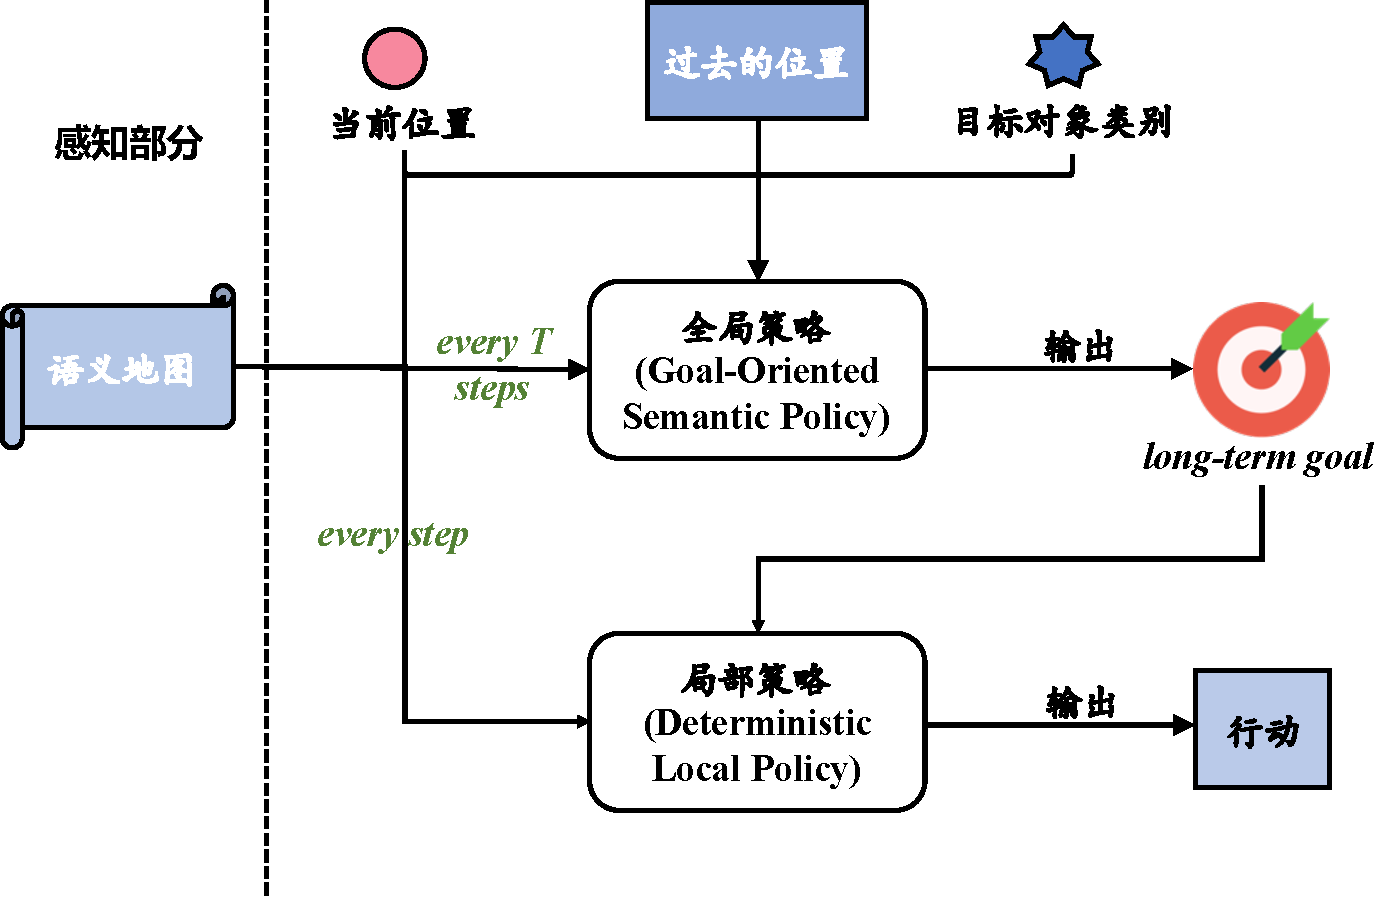
\includegraphics[width=11cm]{assets/policy_structure.pdf}
    \note{
        决策部分可以大致分为两个部分:全局决策和局部决策
        \begin{itemize}
            \item 全局决策:得到长期目标 (\emph{long-term goal})
                  \begin{itemize}
                      \item 输入:已探索真相语义地图与预测的补全语义地图的拼接,语义目标
                      \item coarse time scale: 每T步更新一次long-term goal(减少复杂度)
                      \item 使用CNN以及强化学习(强化学习的reward结合过去的位置确定)
                      \item 决策接下来T步局部决策的目标到达位置
                  \end{itemize}
            \item 局部决策:得到抵达long-term goal的路径 (path)
                  \begin{itemize}
                      \item 输入:语义地图,当前位置,long-term goal
                      \item 也就知道了当前应该采取的行动$a_t$
                      \item fine time scale: 每一步都需要决策
                      \item 采用Far Marching Method~\cite*{...}
                  \end{itemize}
        \end{itemize}
    }
\end{frame}

\subsection{局部决策}
\begin{frame}{局部决策}
    对于局部决策,我们参考~\cite*{chaplot2020object},采用Far Marching Method:
    \begin{itemize}
        \item 利用语义地图中的obstacle channel即可
        \item 和Dijkstra算法类似,通过求解Eikonal方程来更新最短路径:
              $$
                  \begin{aligned}
                      \mid\nabla u(x)\mid & =1/f(x) & \text{for } & x\in\Omega         \\
                      u(x)                & =0      & \text{for } & x\in\partial\Omega
                  \end{aligned}
              $$
    \end{itemize}
\end{frame}

\subsection{全局决策}
\begin{frame}{全局决策}
    \centering
    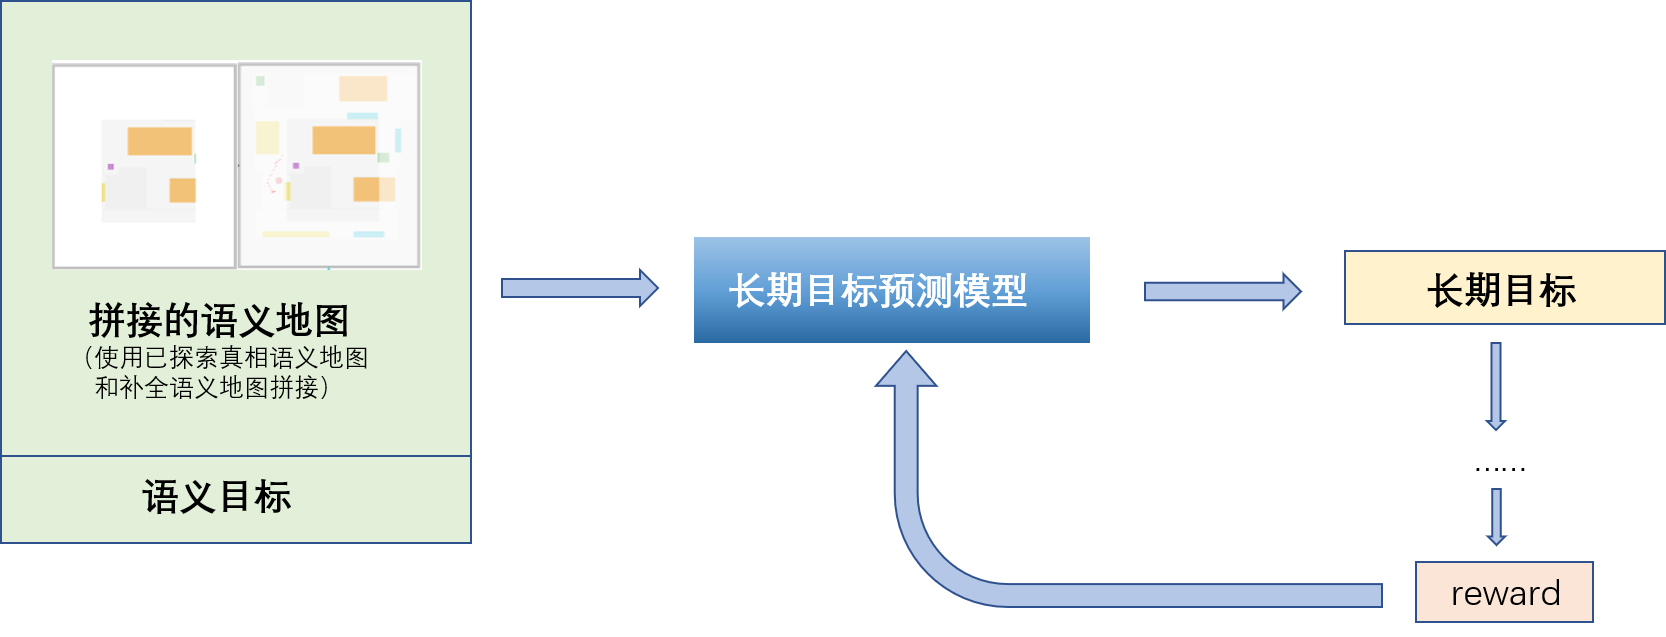
\includegraphics[width=11cm]{assets/global_policy2.png}
    \begin{itemize}
        \item 训练样本真相目标位置的获取:
              \begin{itemize}
                  \item 模拟器提供的全部语义地图
                  \item 语义分割对比技术
              \end{itemize}
    \end{itemize}
    \note{
        \footnotesize
        对于全局决策,我们使用CNN进行一个全局目标的预测。
        \begin{itemize}
            \item 采用CNN预测可能的一个长期目标位置。
            \item 输入:真相语义地图和预测的补全语义地图的拼接,语义目标; 输出:长期目标位置。
            \item 真相目标位置的获取:与感知任务部分所讲类似,使用模拟器或环境绘制提供的全部语义地图以及语义分割对比技术确定。
            \item 与我们参考的论文[16]相比,我们接收已探索的真相语义地图和预测的补全语义地图的拼接作为输入,扩展了CNN的通道数。
            \item 为提高效率,降低复杂度,采用粗粒度时间预测(经过T步行动进行一次长期目标的选择)。(T参考论文[16]使用25)。
            \item 模型进一步采用输入当前位置以及前一时刻位置,用距最近目标物体的距离变化作为reward进行强化学习。
        \end{itemize}
    }
\end{frame}